\subsection{Holographic Pipeline}
\label{sec.holographic_pipeline}

The main pipeline presented in Section~\ref{sec.visualization_pipeline} follows the sequence of transforms: $M_{model}$, $M_{view}$, $M_{proj}$ and $M_{screen}$. In ordinary HCP, $M_{model}$ setups the scene. $M_{view}$ applies the viewpoint of the tracked position, and $M_{proj}$ sets the depth cues. The 3D viewing transforms, $M_{view}$ and $M_{proj}$ can be further split into smaller transforms: a \emph{view pipeline} and  a \emph{projection pipeline}, respectively.

In the proposed FTVR, the screens are tilted to create the virtual screen. The transformation matrix for the tilted screen-local coordinates, $M_{tilt}$, maps the Cartesian coordinate system of the virtual screen onto the screen space coordinate system. If a point is lying in the virtual plane, then the transformation $M_{tilt}$ will realign it to lie into the plane of the screen. The screen space basis are the vectors $v_r$, $v_u$, and $v_n$, the vectors for the right, up and normal directions. The mapping of $M_{tilt}$ is the inverse of the holographic mapping into the plane of the virtual screen. In the holographic views, any point lying in the plane of the screen will be realigned to lie in the virtual screen plane. This mapping is produced by the inverse of $M_{tilt}$. Fortunately, $M_{tilt}$ is an orthogonal rotation, and its inverse is its transpose, $M_{tilt}^{T}$, with screen space basis vectors as rows instead of as columns:

\begin{equation}
\begin{aligned}
M_{tilt}^{T} &= 
\begin{pmatrix} 
v_{rx} & v_{ry} & v_{rz} & 0\\
v_{ux} & v_{uy} & v_{uz} & 0\\
v_{nx} & v_{ny} & v_{nz} & 0\\
0      & 0      & 0      & 1\\
\end{pmatrix}
\end{aligned}
\label{eq.tilt_matrix_transpose}
\end{equation}

The viewpoint of the viewer, $M_{cam}$, simulates a camera looking towards $-z$ with an offset towards $+z$. While the viewpoint can be applied anywhere in the 3D space, the mathematics of perspective projection as defined by matrix $M_{proj}$ disallow this, by the foreshortening division by $z$. The frustum of the camera is forever trapped at the origin, and if we wish to transform the viewpoint, we must instead apply the inverse of this transform to the entire scene. Thus, we instead align the scene with the frustum of the camera. The viewpoint of $M_{cam}$ has to be in tracked position $p_e$, then the scene is translated using the offset of the tracked position to the apex of the frustum. The apex of the perspective frustum is necessarily at zero, thus we translate by $-p_e$ along the vector from the eye:

\begin{equation}
\begin{aligned}
M_{cam} &= 
\begin{pmatrix} 
0      & 0      & 0      & -p_{ex}\\
0      & 0      & 0      & -p_{ey}\\
0      & 0      & 0      & -p_{ez}\\
0      & 0      & 0      & 1\\
\end{pmatrix}
\end{aligned}
\label{eq.camera_matrix}
\end{equation}

For the proposed HCP, the standard perspective transform is set as $M_{hcp}$. This transform have the same parallax for any convergence point in the plane of virtual screen. The near and far distances that composes $M_{hcp}$ are respectively set to the distances to: the plane of virtual screen and the center of the juxtaposition of the physical screens. 

The visualization pipeline for the left and right screens introduces independent transformations for each screen defined by projection transformations for each screen. In usual cases, those projection transformations are used to create a wall composed by many screens with a single vanishing point. The left and right distances in $M_{hcp}$ are displaced by an offset $s_o$. This offset transform $M_{off}$ is applied to $M_{hcp}$ in the projective pipeline $M_{proj} = M_{off} * M_{hcp}$. In this pipeline,  $M_{hcp}$ transforms the scene coordinates to in NDC, as shown in Section~\ref{sec.visualization_pipeline}. Therefore the offsets for half screen to the left and right are $s_{ox} = -1$ and $s_{ox} = 1$, respectively. The offset transform $M_{off}$ have same form as $M_{eye}$, in Equation~\ref{eq.camera_matrix}, and is obtained replacing $p_e$ by $s_o$.

In stereo visualization, the binocular parallax is obtained with the composition of $M_{eye}$ and $M_{stereo}$, Equations~\ref{eq.stereo_view_matrix}and~\ref{eq.stereo_proj_matrix}, in the view and projection pipelines. The view pipeline is the combination of the three transforms: $M_{view} = M_{eye} * M_{tilt}^{T} * M_{cam}$. The plane of the virtual screen has a constant negative parallax at any convergence point in order to simulate the effect of Pepper's Ghost, as proposed in Section~\ref{sec.holographic_emulation}.  The shear transformation of $M_{stereo}$, Equation~\ref{eq.stereo_proj_matrix}, combined with a fixed offset $s_{oz}$ in $M_{off}$ creates the constant negative parallax in the virtual screen. Thus, the projection pipeline becomes the combination of the three transforms: $M_{proj} = M_{stereo} * M_{off} * M_{hcp}$. 

The stereo polarization each side of the left and right stereo pairs in Figures~\ref{fig.split_screens}a-b shows the views as projected in the virtual screen.

\begin{figure}[!hbt]
\centering
\begin{tabular}{cc}
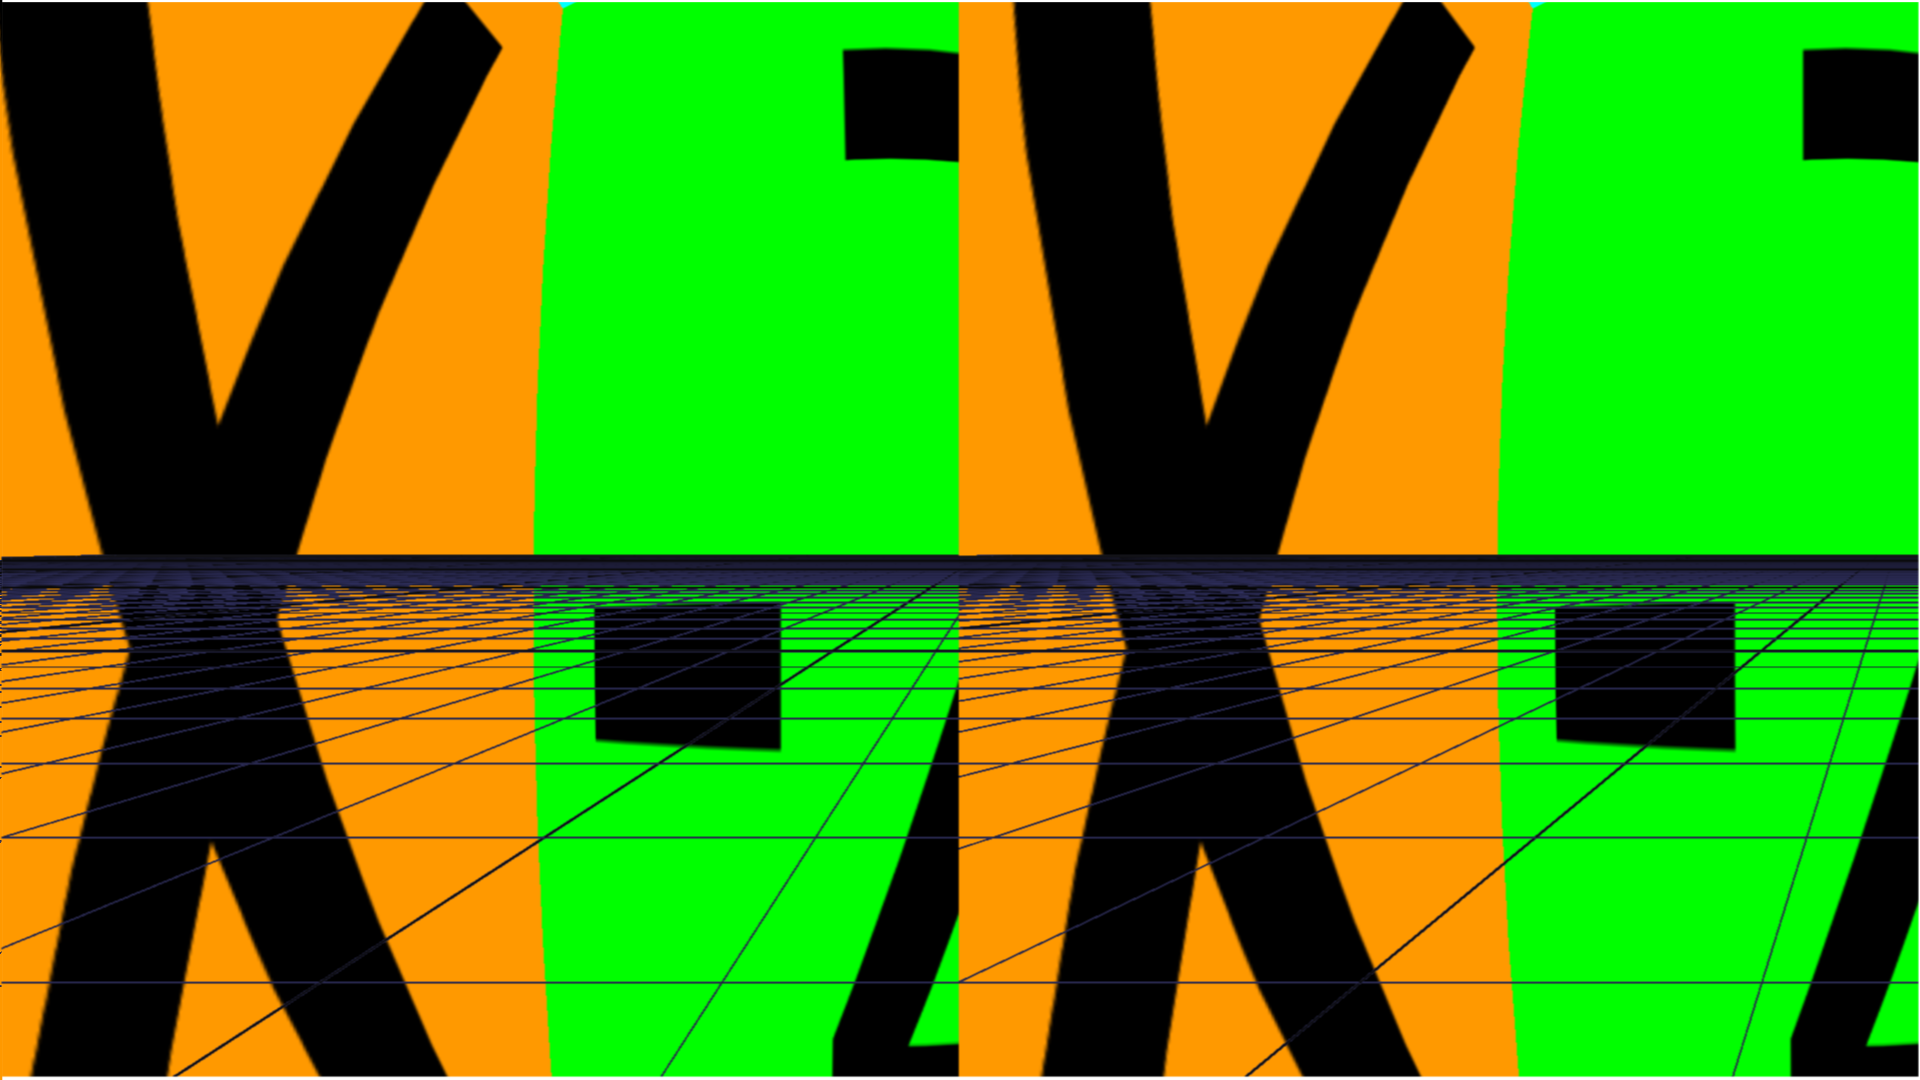
\includegraphics[width=0.45\linewidth,keepaspectratio=true]{figs/left_screen.png}&
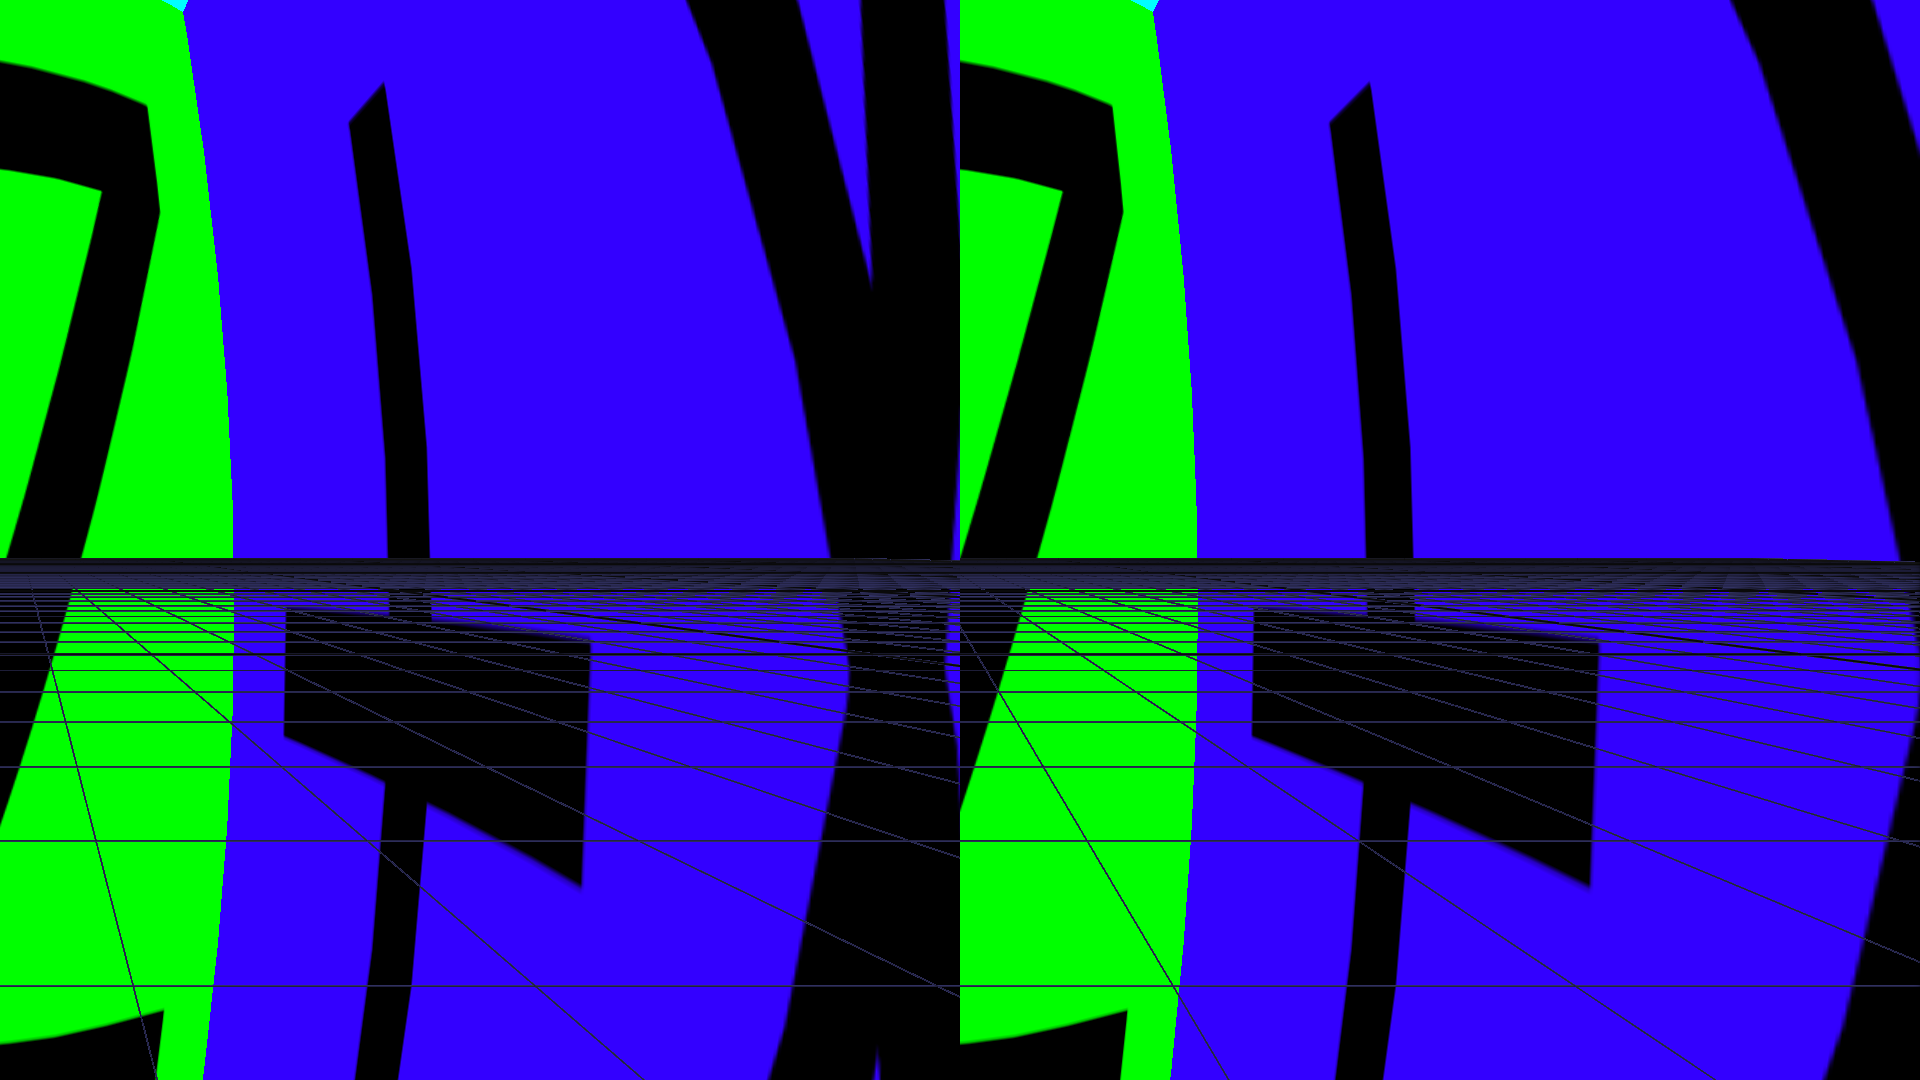
\includegraphics[width=0.45\linewidth,keepaspectratio=true]{figs/right_screen.png}\\
(a) Left display & 
(b) Right display
\end{tabular}
\caption{Vertical split of the stereo views.}
\label{fig.split_screens}
\end{figure}

The complete pipeline is described by Figure~\ref{fig.osg_pipeline}, where each box is a transformation. The bigger boxes are the view and projection transforms, $M_{cam}$ and  $M_{hcp}$, common for both screens. The smaller boxes are the transformations that specific for each screen and have different parameters, $M_{eye}$ and $M_{tilt}^{T}$ after $M_{cam}$; $M_{stereo}$ and $M_{off}$ after $M_{hcp}$.

\begin{figure}[!htb]
\centering
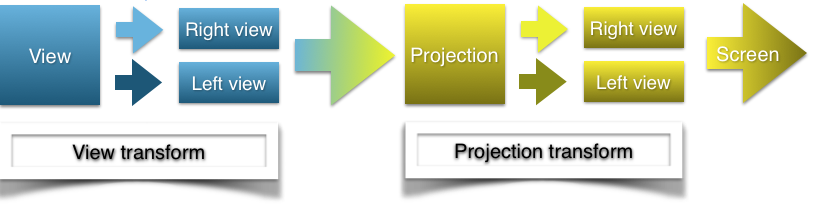
\includegraphics[width=0.9\linewidth,keepaspectratio=true]{figs/osg_pipeline.png}
\caption{The complete pipeline of OpenSceneGraph.}
\label{fig.osg_pipeline}
\end{figure}